%%This is a very basic article template.
%%There is just one section and two subsections.
\documentclass{article}
\usepackage[utf8]{inputenc}              	%nastaven� v�choz�ho k�dov�n� textu
\usepackage[czech]{babel}                	%nastaven� �esk�ch znak�
\usepackage[pdftex]{graphicx}				%umo��uje vkl�d�n� obr�zk� v jpg, png
\usepackage{amsfonts}						%package obsahujici symboly mnozin treba - \mathbb{N}
%\usepackage{amssymb}						%stejna funkce jako amsfonts				%stejna funkce jako amsfonts

\begin{document}
\section{Validátory}
Vzhledem k některým guardům, které nemapují entity, pokud je model v
nekonzistentním stavu jsme se rozhodli pro vytvoření validačního query, které
zkontroluje stav modelu. Toto query se dá použít na vstupní  i výstupní model.

\section{Validátor aplikačního modelu}
Nekonzistentní stavy modelu se dělí do těchto kategorií:
\begin{itemize}
  \item duplicitní jména(Class, property, \ldots)
  \item hierarchie dědičnosti
  \item primitivní typy
  \item vazby
  \item embeddedClass
\end{itemize}

\subsection{Duplicitní jména}
Neexistuje Class v generaci se jménem shodným s jménem jiné třídy v téže
generaci \newline

Neexistuje property ve třídě se shodným jménem s property téže třídy nebo jejího
předka

\subsection{hierarchie ddičnosti}
Neexistuje abstraktní třída, která by měla neabstraktního parenta\newline

Neexistuje třída, která by sobě samé byla předkem ( v hierarchii nevzniká
cyklus)

\subsection{Primitivní tridy}
Neexistuje primitivní třída, která by měla id

\subsection{Property}
Neexistuje třída, která by měla property neprimitivního typu, jejíž opposite
property by nebyla nastavená původní property. //to chce prepsat

Všechny primitivní Property mají nastavenou oppositeProperty na null 

\subsection{EmbeddedClass}
Neexistuje embeddedClass v generaci, která by měla property jiné arrity než
0 \ldots 1 x 1 nebo 1 x 1 \newline

V rámci třídy neexistuje Property v hierarchii, která by měla name shodné s
Stringem reprezentujícím property typu EmbeddedTřída. Poznámka: reprezentativní
Stringy property se rovnají:\newline
 property.name + "\_" + property.type.property[i].name \newline

Na obr. \ref{pict:embedded-collision} vidíme příklad takové kolize jmen.
Reprezentativními Stringy jsou "income\_amount" a "income\_currency", které jsou
v kolizi s jménem property třídy Person. Druhou chybou je multiplicita M x N.
\begin{figure}[t]
	\begin{center}
	\refstepcounter{figure}
	\label{pict:embedded-collision}		             
    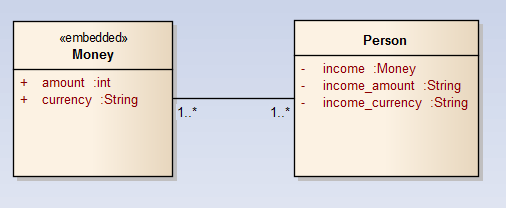
\includegraphics[scale=1.0]{../images/embedded_collision_example.png}
	\caption{EmbeddedClass kolize}
	\end{center}			     
\end{figure}


\end{document}
